\chapter{Knowledge gain with multiple episodes}
\begin{quotation}
\noindent ``\emph{quote}''
\begin{flushright}\textbf{author}\end{flushright}
\end{quotation}

We will first and foremost analyse how a reinforcement learning agent 
performs when it is confronted to playing a single episode of one of the 
CartPole problems. We will train the agent on a distribution of 20 permutations
(shown on Table~\ref{tab:20perms}), at first without inverting the agent's
action.

\begin{table}
	\centering
	\caption{State permutations used for training and testing}
	\label{tab:20perms}
	\subfloat[Training distribution]{
		\bgroup
		\def\arraystretch{1.5}
		\begin{tabular}{c|c|c}
			[0, 1, 2, 3] & [1, 0, 2, 3] & [2, 0, 1, 3] \\
			\hline
			[0, 1, 3, 2] & [1, 0, 3, 2] & [2, 0, 3, 1] \\
			\hline
			[0, 2, 1, 3] & [1, 2, 0, 3] & [2, 1, 0, 3] \\
			\hline
			[0, 2, 3, 1] & [1, 2, 3, 0] & [3, 0, 1, 2] \\
			\hline
			[0, 3, 1, 2] & [1, 3, 0, 2] & [3, 0, 2, 1] \\
			\hline
			[0, 3, 2, 1] & [1, 3, 2, 0] & [3, 1, 0, 2] 
		\end{tabular}
		\egroup
	}
	\subfloat[Testing distribution]{
		\quad\quad
		\bgroup
		\def\arraystretch{1.5}
		\begin{tabular}{c}
			[2, 1, 3, 0] \\
			\hline
			[2, 3, 0, 1] \\
			\hline
			[2, 3, 1, 0] \\
			\hline
			[3, 1, 2, 0] \\
			\hline
			[3, 2, 0, 1] \\
			\hline
			[3, 2, 1, 0]
		\end{tabular}
		\egroup
		\quad\quad
	}
\end{table}

Surprisingly, the agent manages to reach a very good performance level, only
failing...

\begin{figure}
	\centering
	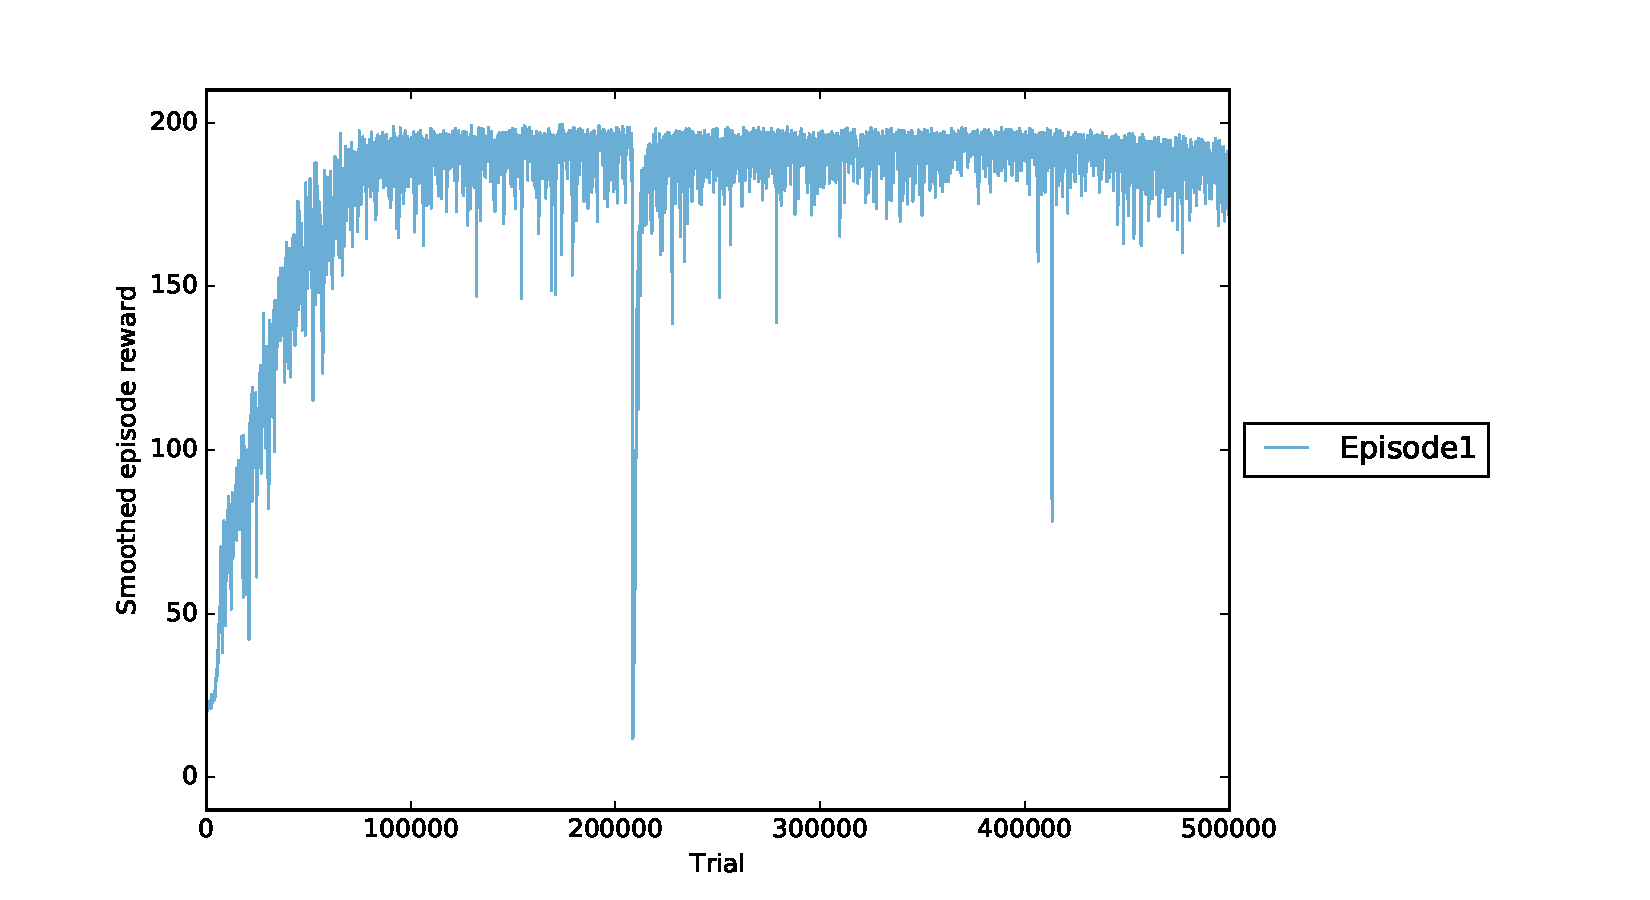
\includegraphics[width=0.9\linewidth]{fig/20perms1ep_training.pdf}
	\caption{Training of an agent on trials of 1 episode}
	\label{fig:20perms1ep_training}
\end{figure}

does making it play for several episodes improve performance?

\begin{figure}
	\centering
	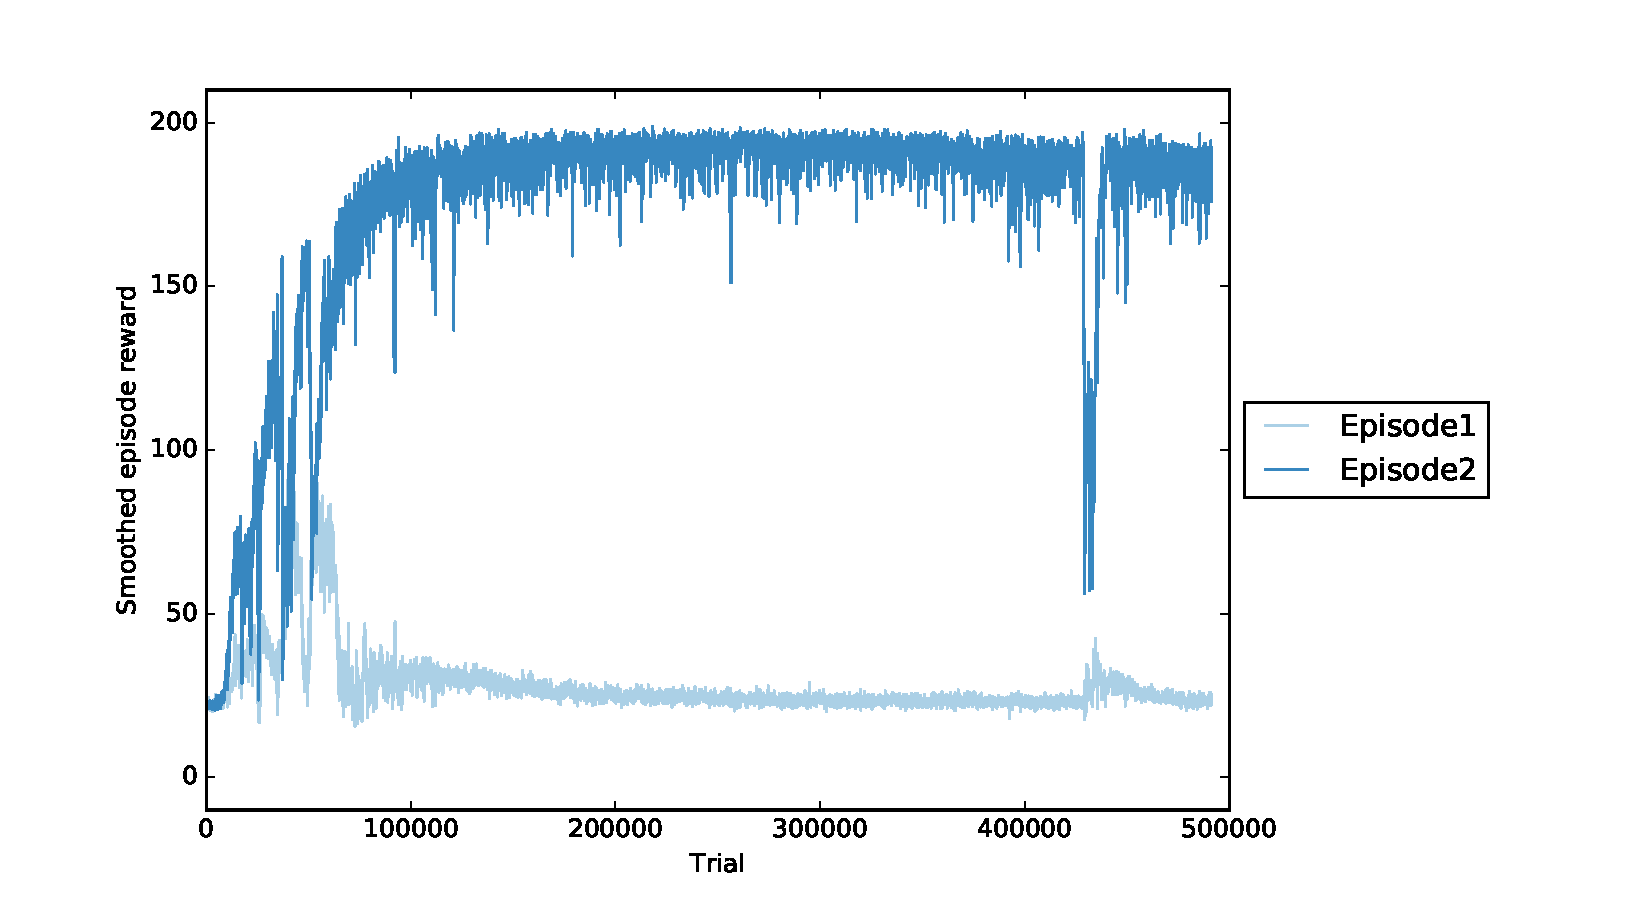
\includegraphics[width=0.9\linewidth]{fig/20perms2ep_training.pdf}
	\caption{Training of an agent on trials of 2 episodes}
	\label{fig:20perms1ep_training}
\end{figure}

Immediately, we see first episode be bad. Why? Discussion of this in section
with structure reward etc

However only seeing the avg reward of second episode doesn't give us enough
info

But if we compare distributions of rewards for last episode, we see one 
performs better than the other. (make clear it's only for seen distributions)

\begin{figure}
	\centering
	\subfloat[][Trials of 1 episode]{
		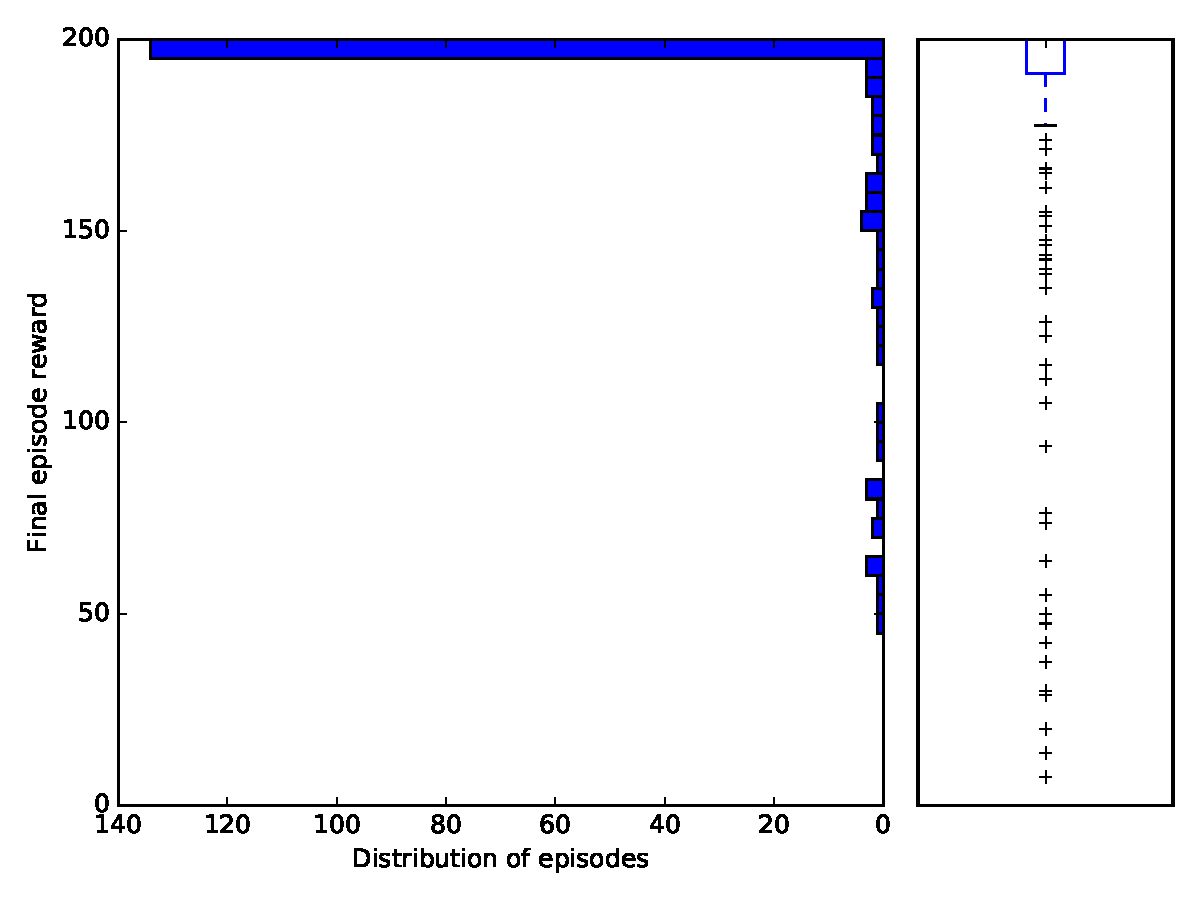
\includegraphics[width=0.49\linewidth]{fig/20perms_distrib_1ep.pdf}}
	\subfloat[][Trials of 2 episodes]{
		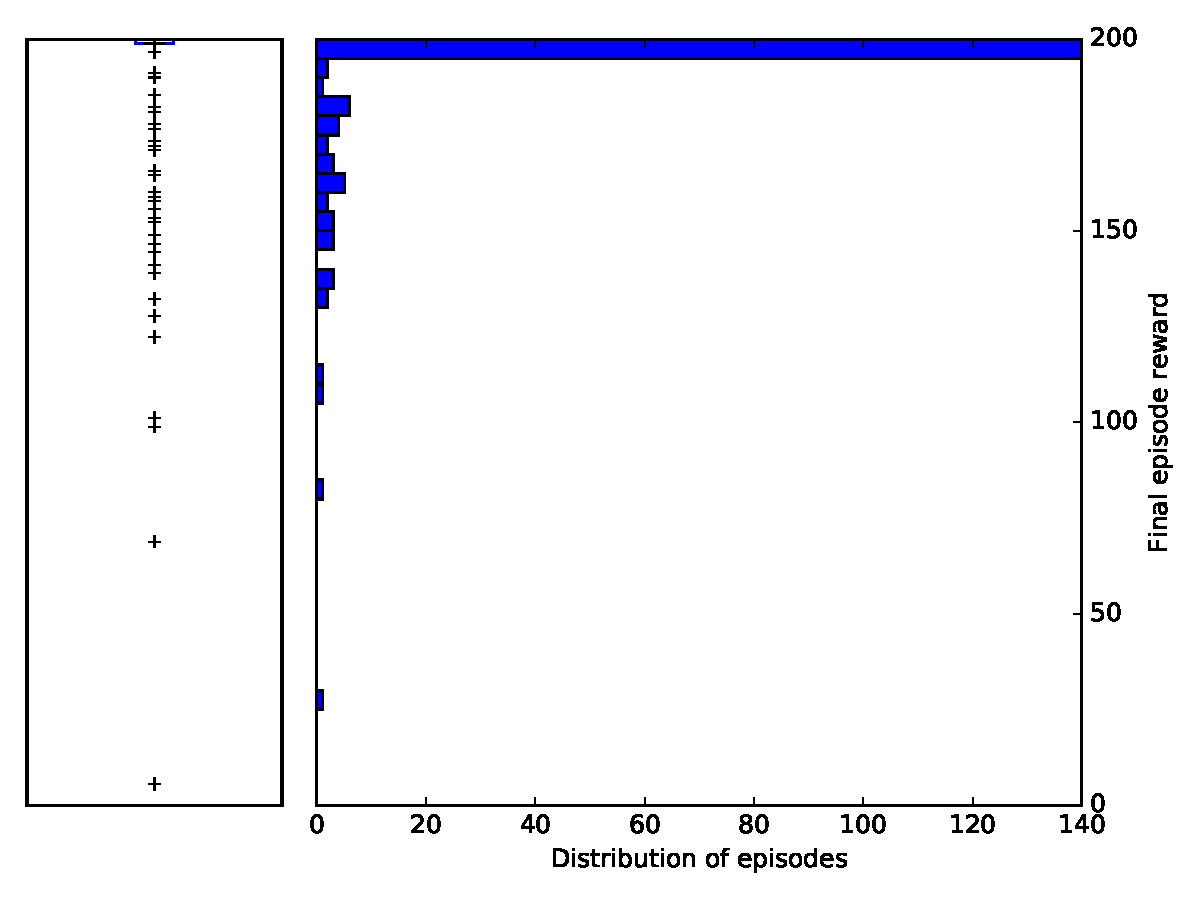
\includegraphics[width=0.49\linewidth]{fig/20perms_distrib_2ep.pdf}}
	\caption{}
	\label{fig:20perms_distrib}
\end{figure}
This is even clearer for unseen permutations.

\begin{figure}
	\centering
	\subfloat[][Trials of 1 episode]{
		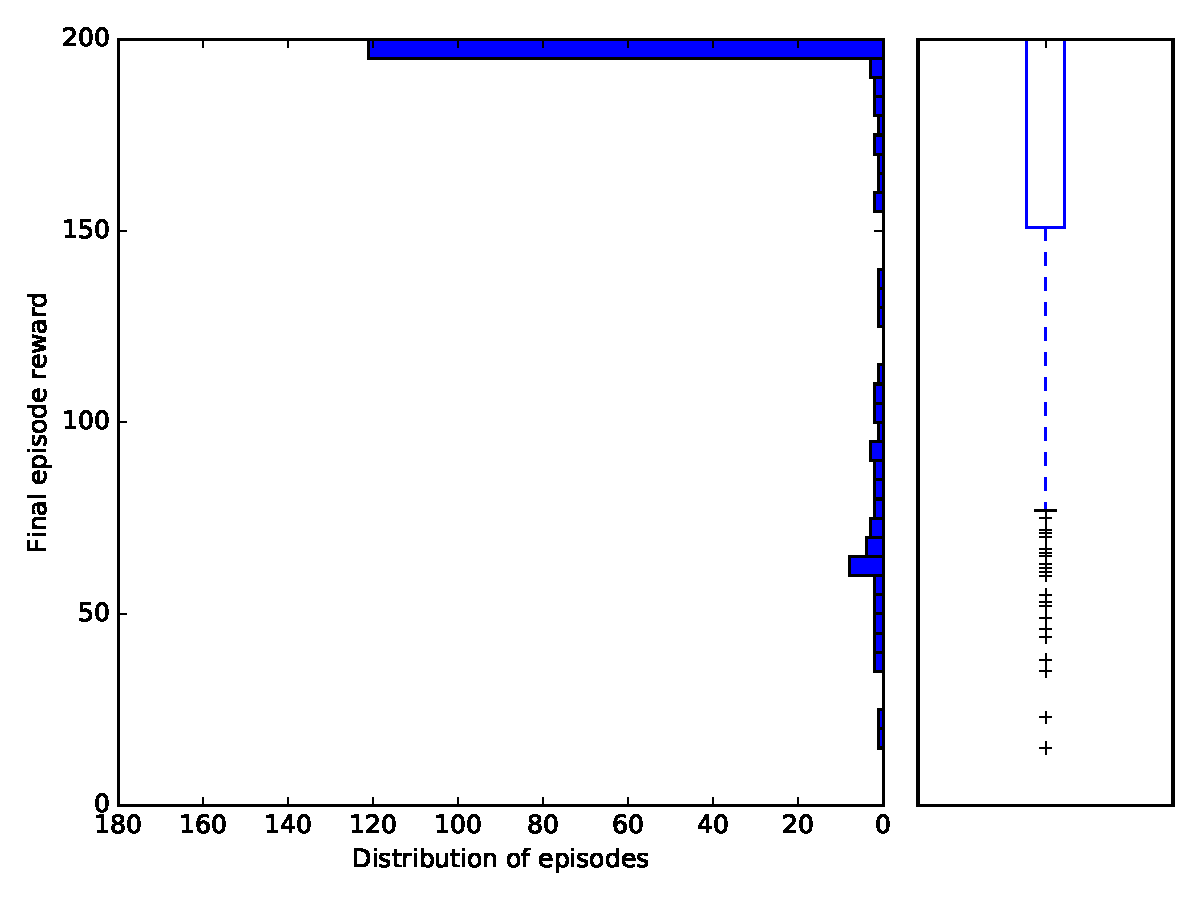
\includegraphics[width=0.49\linewidth]{fig/20perms_unseen_distrib_1ep.pdf}}
	\subfloat[][Trials of 2 episodes]{
		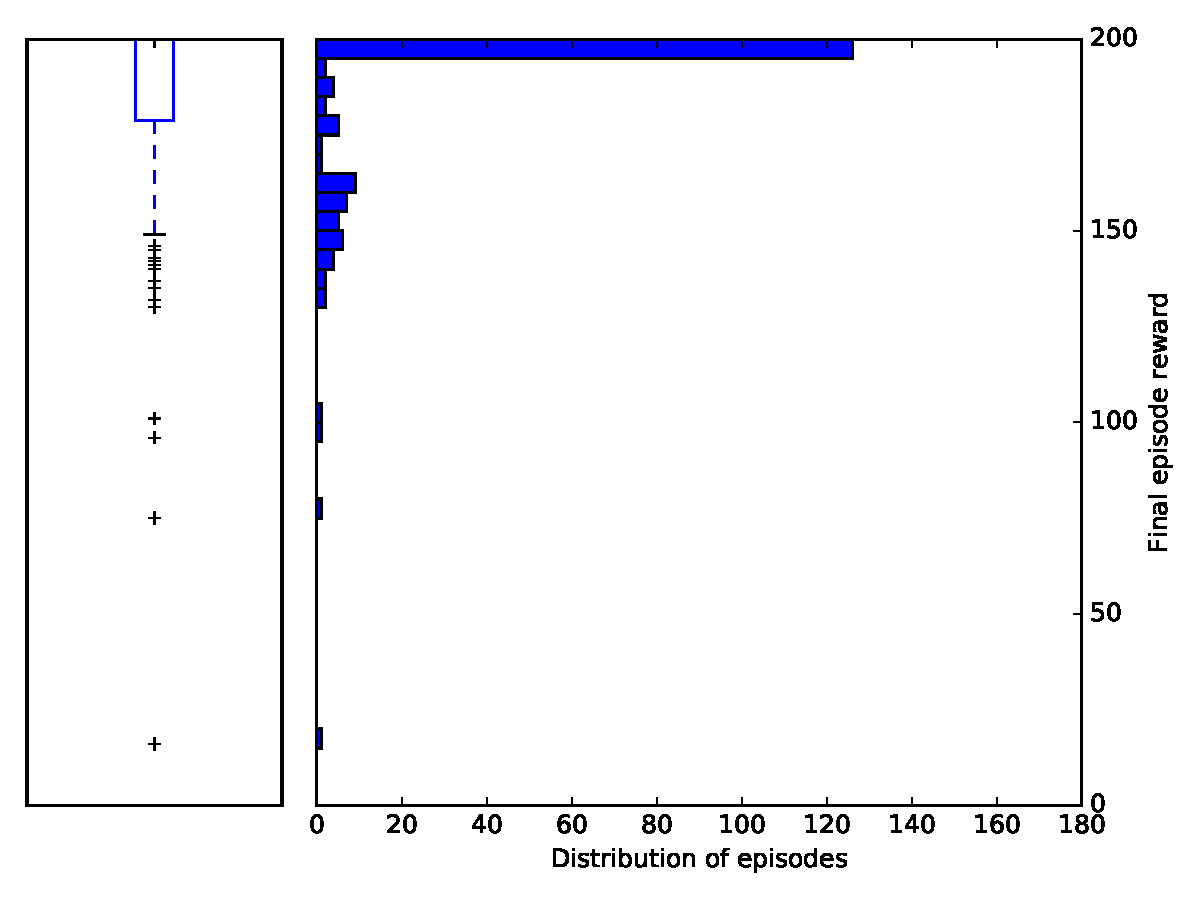
\includegraphics[width=0.49\linewidth]{fig/20perms_unseen_distrib_2ep.pdf}}
	\caption{}
	\label{fig:20perms_unseen_distrib}
\end{figure}

If we add the left-right confusion, this effect is magnified
\begin{figure}
	\centering
	\subfloat[][Trials of 1 episode]{
		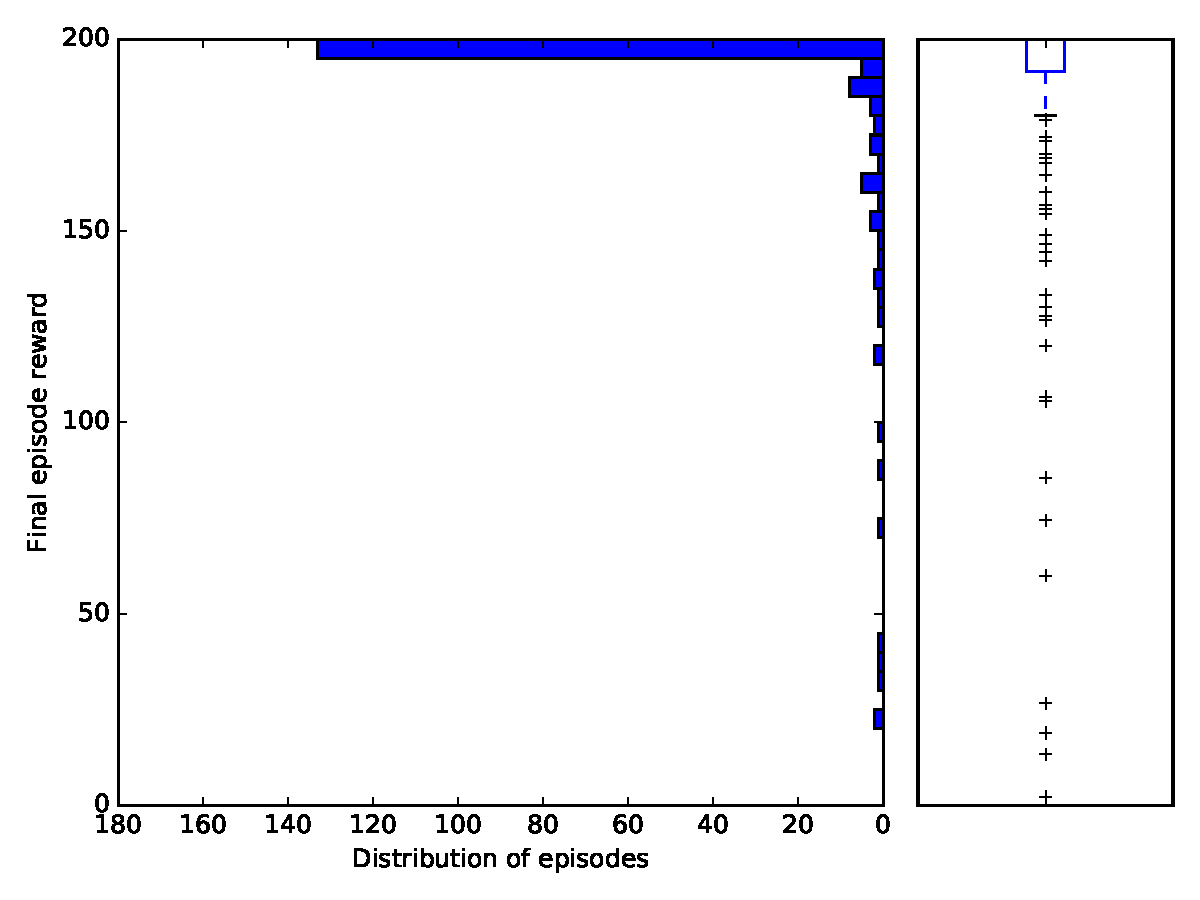
\includegraphics[width=0.49\linewidth]{fig/20permsLR_distrib_1ep.pdf}}
	\subfloat[][Trials of 2 episodes]{
		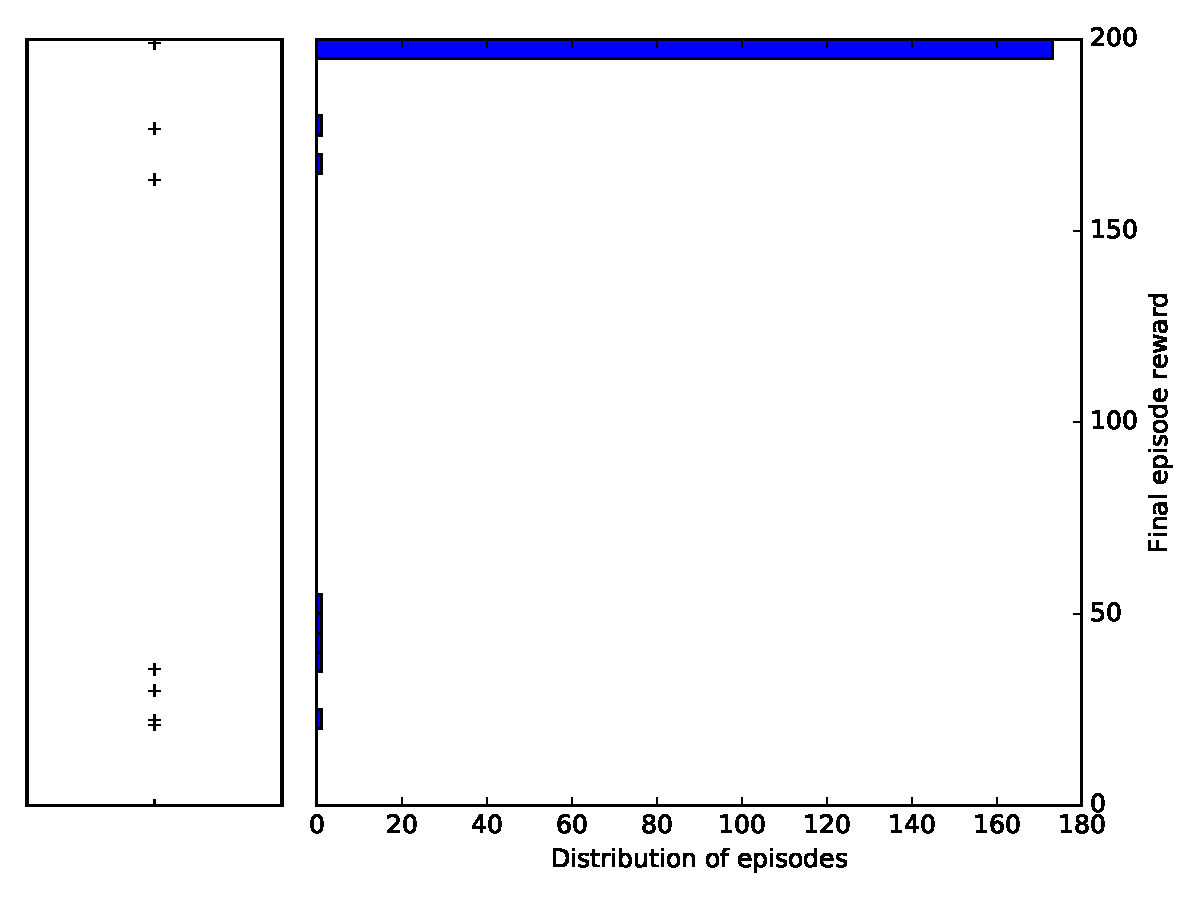
\includegraphics[width=0.49\linewidth]{fig/20permsLR_distrib_2ep.pdf}}
	\caption{}
	\label{fig:20permsLR_distrib}
\end{figure}

Once again, even more so when confronted to unseen permutations.
\begin{figure}
	\centering
	\subfloat[][Trials of 1 episode]{
		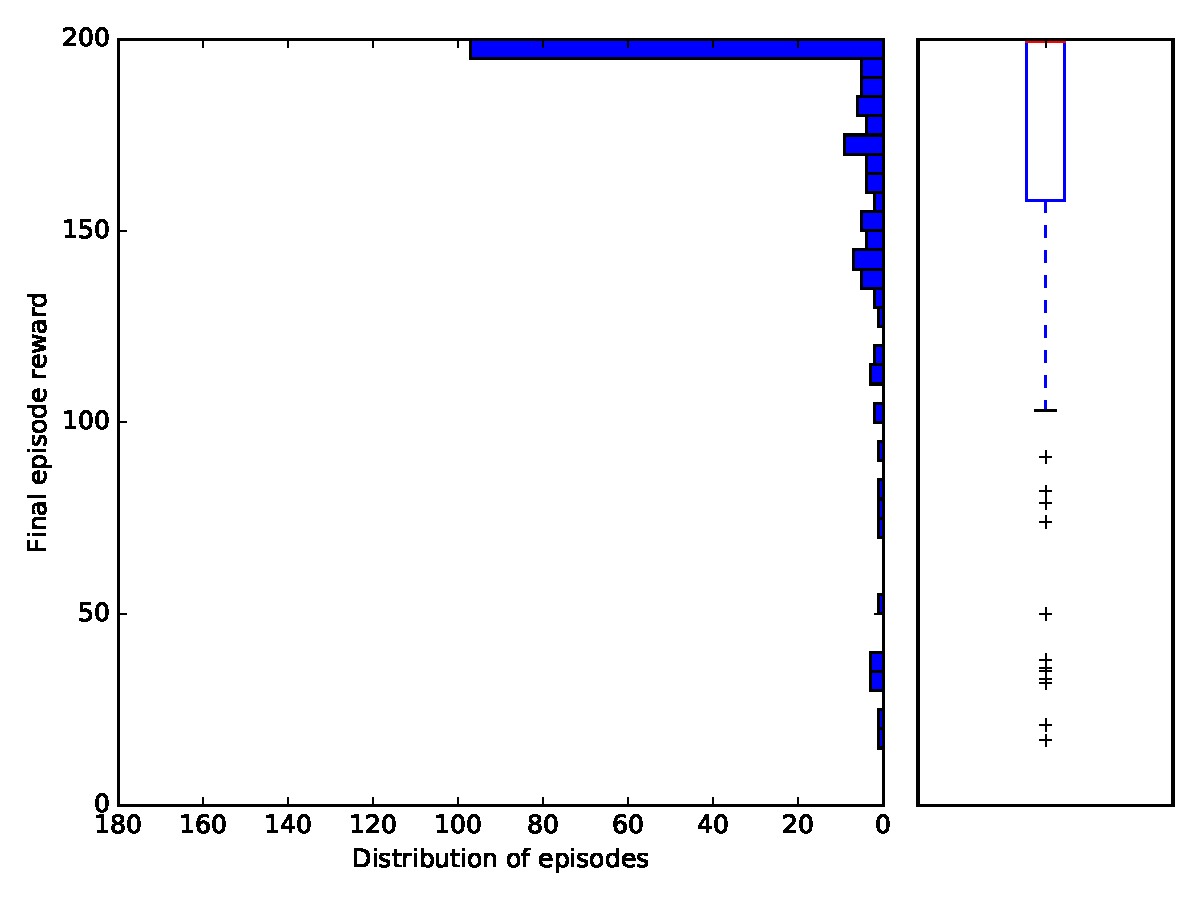
\includegraphics[width=0.49\linewidth]{fig/20permsLR_unseen_distrib_1ep.pdf}}
	\subfloat[][Trials of 2 episodes]{
		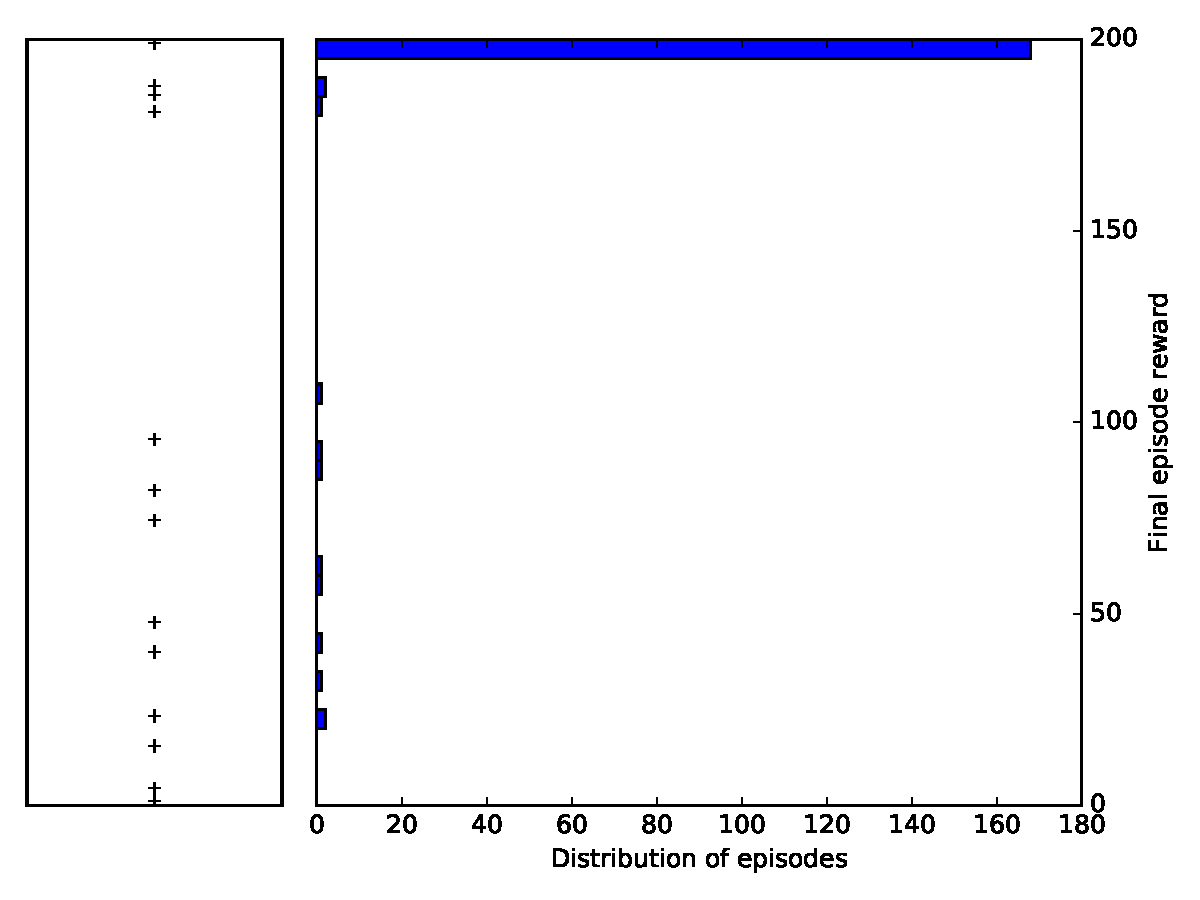
\includegraphics[width=0.49\linewidth]{fig/20permsLR_unseen_distrib_2ep.pdf}}
	\caption{}
	\label{fig:20permsLR_unseen_distrib}
\end{figure}






